\documentclass[10pt]{article}

\usepackage{amsmath}

\newcommand{\myvec}[1]{\ensuremath{\begin{pmatrix}#1\end{pmatrix}}}

\newcommand{\mydet}[1]{\ensuremath{\begin{vmatrix}#1\end{vmatrix}}}

\newcommand{\solution}{\noindent \textbf{Solution: }}

\providecommand{\brak}[1]{\ensuremath{\left(#1\right)}}

\providecommand{\norm}[1]{\left\lVert#1\right\rVert}
\usepackage{graphicx}
\usepackage{float}

\let\vec\mathbf
\title{Coordinate-Geomentry}
\title{Coordinate Geometry}
\author{adityatanish.chakka@sriprakashschools.com}

\begin{document}
\maketitle
\section*{Class 10$^{th}$ Maths - Chapter 7}
This is Problem-10 from Exercise 7.2
\begin{enumerate}
\item Find the area of the rhombus whose vertices are:
(3,0),(4,5),(-1,4),(-2,-1)
\begin{align}
{(3,0),(4,5),(-1,4),(-2,-1)}
\end{align}
\solution \\

Given Data:
\begin{align}
\vec{A} = \myvec{3\\0}\\
\vec{B} = \myvec{4\\5}\\
\vec{C} = \myvec{-1\\4}\\
\vec{D} = \myvec{-2\\-1}\\
\end{align}
\begin{align}
\vec{BA} = \myvec{-1\\-5}\\
\vec{DA} = \myvec{5\\1}\\
\vec{CB} = \myvec{5\\1}\\
\vec{DB} = \myvec{6\\6}\\
\end{align}
AREA OF A RHOMBUS;
\begin{align}
\frac{1}{2}\norm{\vec{A}-\vec{B}\times \vec{A}-\vec{D}}+\frac{1}{2}\norm{\vec{B}-\vec{C}\times \vec{B}-\vec{D}}\\
\frac{1}{2}\mydet{-1 & 5\\ -5 & 1}+\frac{1}{2}\mydet{5 & 6\\ 1 & 6}\\
\frac{1}{2}\norm{-1+25}+\frac{1}{2}\norm{30-6}\\\
\frac{1}{2}\norm{24}+\frac{1}{2}\norm{24}\\
12+12 sq.units\\
24 sq.units\\
\end{align}
therefore the area of the given rhombus is 24 sq.units
\end{enumerate}
\begin{figure}[H]
			\centering
			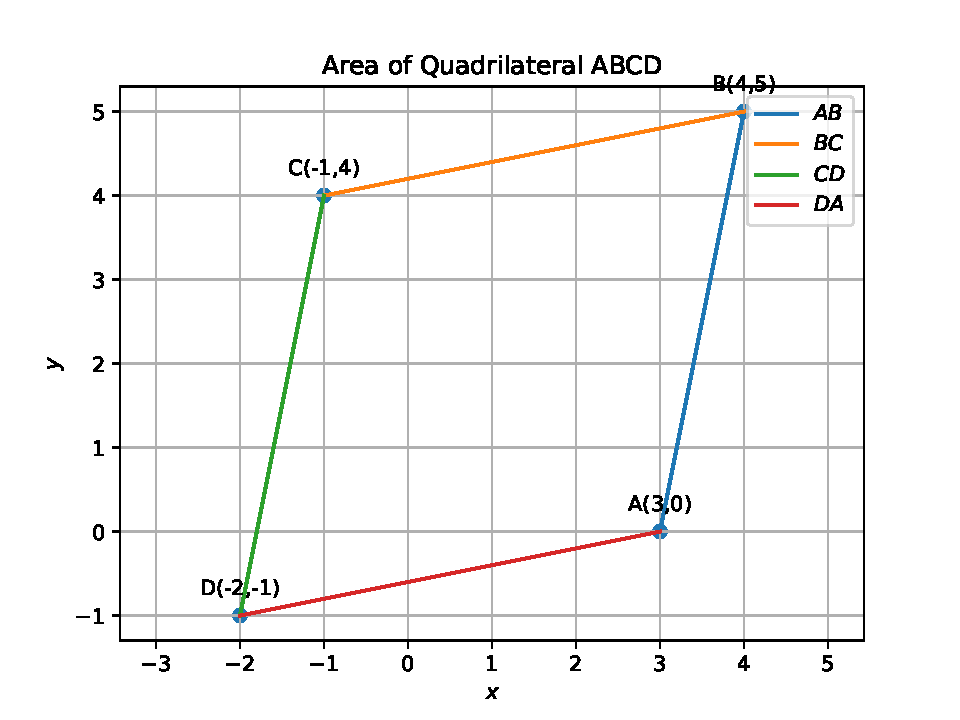
\includegraphics[width=\columnwidth]{figs/fig.pdf}
			\caption{Quadrilateral ABCD}
			\label{fig:15}
		\end{figure}
\end{document}
